\section{Association Analysis} \label{association analysis}

Association rule mining is the task of finding associations between \textit{items} in a database of \textit{transactions}. The technique was originally developed in 1993 to identify patterns in consumers grocery purchasing behaviour. Since then however, association analysis has found applications in wide variety of domains.

Let us consider a hypothetical dataset shown in table~\ref{table:raw-data}. The dataset consists of mobile device system settings and energy usage measurements. The dataset has three continuous valued variables:  energyRate, the rate at which the battery is discharging;  CPULevel, the device's CPU usage level and screenBrightness, the brightness of the device's screen. Each of these variables takes floating point values ranging from 0 to 1.
\begin{table}[htb]
    \begin{tabular}{ | l | l | l | }
    \hline
    \textbf{energyRate} & \textbf{CPULevel} & \textbf{screenBrightness} \\ \hline
    0.21 & 0.58 & 0.30 \\ \hline 
    0.80 & 0.46 & 0.61 \\ \hline 
    0.76 & 0.65 & 0.93 \\ \hline 
    0.58 & 0.99 & 0.54 \\ \hline 
    \end{tabular}
	\caption{Hypothetical mobile device measurements inspired by Carat dataset}
	\label{table:raw-data}
\end{table}

Since association rule mining requires each variable of the database to be binary valued, a discretization of the variables must be performed. To discretize a continuously valued variable, we need to replace the continuous variable with multiple binary valued variables, each corresponding to an interval or cluster of values of the continuous variable. The details of discretization are discussed in chapter ???. For now, let us consider a naive discretization strategy, where each continuous variable is split to two binary variables by creating two bins at cut point 0.5. Table~\ref{table:discreteData} demonstrates this idea.

\begin{table}[htb]
    \begin{tabular}{ | l | l | l | l | l | l | }
    \hline
    \textbf{energy=low} & \textbf{energy=high} & \textbf{CPU=low} & \textbf{CPU=high} & \textbf{screen=low} & \textbf{screen=high} \\ \hline
    True & False & False & True & True & False \\ \hline 
    False & True & True & False & False & True \\ \hline 
    False & True & False & True & False & True \\ \hline 
    False & True & False & True & False & True \\ \hline 
    \end{tabular}
	\caption{Hypothetical mobile device measurements after naive discretization}
	\label{table:discreteData}
\end{table}

Since every group of variables that is created by discretization is mutually exclusive, a more concise notation for this dataset can be used, as shown in table~\ref{table:discreteDataConcise}.

\begin{table}[htb]
    \begin{tabular}{ | l | l | l |}
    \hline
	\textbf{energyRate} & \textbf{CPULevel} & \textbf{screenBrightness} \\ \hline
    low & high & low  \\ \hline 
    high & low & high \\ \hline 
    high & high & high \\ \hline 
    high & high & high \\ \hline 
    \end{tabular}
    \caption{Hypothetical mobile device measurements after discretization using concise notation}
    \label{table:discreteDataConcise}
\end{table} 

%As an example, consider a hypothetical database of following transactions denoting individual mobile device system settings, extracted from the Carat data:
 
%\begin{center}
%    \begin{tabular}{ | l | l | }
%    \hline
%    \textbf{Items} \\ \hline
%    cpuLevel=high, energyRate=high \\ \hline 
%    diapers, beer, cookies \\ \hline 
%    diapers, beer, bread \\ \hline 
%    butter, bread, cheese \\ \hline 
%    \end{tabular}
%\end{center} 
 
%The goal of the association analysis is then to produce a list of association rules, given a some measure of interestingness. From the database given above, some algorithm might produce the following association rules: 

Having transformed the raw data to binary variables, the goal of the association analysis is then to produce a list of association rules, given some measure of interestingness. For the database given above, an association rule mining algorithm might find the following association rule 

\[
	\left\{ CPULevel=high, screenBrightness=high \right\} \Rightarrow \left\{ energyRate=high \right\}
\]

This rule implies that high CPU utilization together with high screen brightness associates with high level of battery consumption.

\subsection{Formal Problem Definition}

Let $I = \left\{ x_1, x_2, ..., x_n \right\}$ be a set of binary variables called items. A transaction database $T$ is then a multiset of subsets of $I$, where each element of $T$ denotes a transaction. To give the exact problem of association rule discovery, concepts of support and confidence need to be introduced.

Support of an item set $X$ in database $T$ is defined as the fraction of all transactions in $T$ that contain the item set~\cite{Hipp:2000:AAR:360402.360421}.

\[ supp(X) = \dfrac{ \vert \left\{ X' \in T  \mid X \subseteq X'  \right\}  \vert }{ \vert T \vert  } \]

Confidence of a rule $X \Rightarrow Y$, where $X$ and $Y$ are item sets of $T$, is defined as the fraction of transactions in $T$ containing item set $X$ which also contain $Y$~\cite{Hipp:2000:AAR:360402.360421}.

\[conf( X \Rightarrow Y) = \dfrac{ supp( X \bigcup Y ) }{ supp(X) } \]

The problem of association rule discovery can now be formalized the following way. Given a transaction database $T$, minimum support level $s$, where $ 0 \leq s \leq 1 $ and minimum confidence level $c$, where $ 0 \leq c \leq 1 $, find all rules $X \Rightarrow Y$ where $conf( X \Rightarrow Y ) \geq c$, $supp(X) \geq s$ and $supp(Y) \geq s$~\cite{Hipp:2000:AAR:360402.360421}. 

The association rule discovery problem can be further divided into two distinct sub problems, namely frequent pattern mining problem and rule generation problem. A frequent pattern $P$ of database $T$ is a subset of $I$ such that $supp(P) \geq s$. The frequent pattern mining problem is the task of finding all frequent patterns from a given database. The rule generation problem on the other hand, is the task of generating all association rules with sufficient confidence from the frequent patterns. 

\subsection{Frequent Pattern Mining Using Frequent Pattern Growth}

Frequent pattern growth is an efficient algorithm for the frequent pattern mining problem~\cite{Han:2000:MFP:335191.335372}. The algorithm utilizes a specialized data structure called FP-tree, a kind of prefix tree, to speed up the frequent pattern generation. The FP-tree data structure consists of nodes, each of which have tree fields: item name, which tells what item the node represents; item count, which tells the number of transactions containing the item that can be reached by following the path of nodes leading to the node; and node link, which contains a pointer to the next node in the FP-tree with the same node name. An exception is the root node of the FP-tree, which does not have any of these fields, but only has links to child nodes. Algorithm~\ref{Algorithm:FP-tree} shows how to constructs a FP-tree for a transaction database~\cite{Han:2000:MFP:335191.335372}.

\begin{algorithm}[h]
	\SetAlgoLined\DontPrintSemicolon
	\SetKwFunction{buildFPTree}{buildFPTree}\SetKwFunction{insertTree}{insertTree}
	\KwData{A transaction database \textit{DB}, minimum support threshold \textit{s}}
	\KwResult{FP-tree for the database}
	\SetKwProg{myalg}{Algorithm}{}{}
	\myalg{\buildFPTree{}}{
		\nl	\textit{F} $\leftarrow$ Scan \textit{DB} and collect a map of items and their frequencies\;
		\nl \textit{L} $\leftarrow$ Sort keys of \textit{F} in descending order of support filtering out items which have support < \textit{s}\;
		\nl \textit{T} $\leftarrow$ root node of the FP-tree\;
		\nl \For{ transaction \textit{Trans} \textbf{in} \textit{DB} }{ 
			\nl sort \textit{Trans} according to \textit{L} and filter out infrequent items\;
			\nl insertTree(\textit{Trans}, \textit{T})\;
		}
		\nl \KwRet{\textit{T}}\;
	}
	\setcounter{AlgoLine}{0}
	\SetKwProg{myproc}{Procedure}{}{}
  	\myproc{\insertTree{\textit{Trans}, \textit{T}}}{
		\nl \If{\textit{Trans} is empty}{
			\nl \KwRet\;
		} \nl \Else{
			\nl	\textit{N} $\leftarrow$ first item of \textit{Trans}\;
			\nl \textit{tail} $\leftarrow$ tail of \textit{Trans}\;	
			\nl \If{ \textit{T} has a child \textit{N} such that \textit{N}.item-name == \textit{h}.item-name} {
				\nl \textit{N}.count += 1\;
				\nl insertTree(\textit{tail}, \textit{N})
			} \nl \Else {
				\nl \textit{N} $\leftarrow$ create new node with item-name = \textit{p}.item-name and count = 1 and link \textit{T} as its parent\;
				\nl insertTree(\textit{tail}, \textit{N})
			}
		}
	}	
	\caption{Fp-tree construction}
	\label{Algorithm:FP-tree}
\end{algorithm}  

Let us go through the process of building a FP-tree for an example transaction database. First step of building a FP-tree, is to sort each transaction by decreasing order of frequency of its items in the database. Infrequent items are also filtered out based on the minimum support. Table~\ref{table:fp-growth-example1} shows the example transaction database as well as the frequent items in descending order of frequency. A single traversal over the database is required in order to sort the transactions.

For this example, let us consider a minimum support of 0.3. Since the number of transactions in our database is 6 and $ \frac{1}{6} < 0.3 < \frac{2}{6} $, all items with frequency less than 2 can be filtered out. Thus items i and j are not included in the second column of table~\ref{table:fp-growth-example1}. 

\begin{table}[htb]
\begin{center}
    \begin{tabular}{ | l | l | }
    \hline
	\textbf{Items} & \textbf{Frequency Ordered and Filtered Items} \\ \hline
    a, b, c, d, e, h & c, e, h, a, b, d \\ \hline 
    c, d, e, h & c, e, h, d \\ \hline 
    c, e, h & c, e, h \\ \hline 
    a, b, c, e, j & c, e, a, b \\ \hline 
    c, h & c, h \\ \hline
    d, i & d \\ \hline
    \end{tabular}
    \caption{Example transaction database for illustrating FP-tree generation.}
    \label{table:fp-growth-example1}
\end{center}
\end{table} 

To construct the FP-tree we start with a node labled as "root". We then take the first transaction and walk over its elements in the frequency order. We start from the root node of the FP-tree, and since it has no child nodes, we add a child node labelled with "c" and set its count to 1. We then continue to walk from the node labelled with "c" and repeat the procedure for the remaining items of the transaction. The FP-tree after processing the first transaction is shown in figure~\ref{figure:fp-growth-example1}.

\begin{figure}[h]
	\centering
	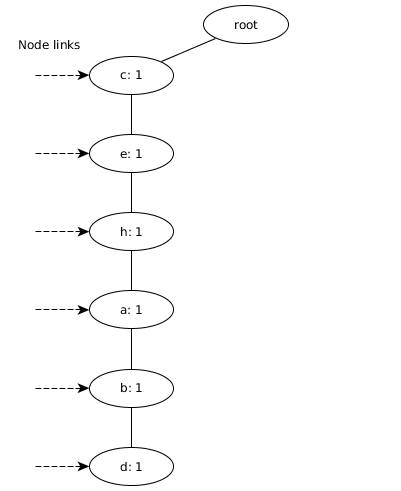
\includegraphics[scale=0.5]{fp-tree-example/fp-tree-p1.png}
	\caption{FP-tree after processing the first transaction}
	\label{figure:fp-growth-example1}
\end{figure}

Next, the second transaction is processed as follows. We again start at the root node and walk over all items in the second transaction. Since the root node has a child node labelled with "c" we simply increment its count to 2. We walk down the path $c \rightarrow e \rightarrow h$ incrementing the counts of these nodes. The next  item to process is "d" and we are at the node labelled with "h". Since the node does not have a child node labelled with "d", we add one and set its count to 1. Figure~\ref{figure:fp-growth-example2} shows the progress of building the FP-tree after processing the second transaction of the database.

\begin{figure}[h]
	\centering
	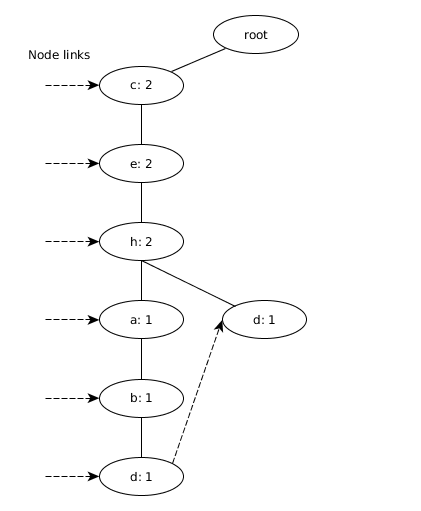
\includegraphics[scale=0.5]{fp-tree-example/fp-tree-p2.png}
	\caption{FP-tree after processing the second transaction}
	\label{figure:fp-growth-example2}
\end{figure}

Repeating the same procedure for the rest of the transactions yields complete FP-tree as illustrated in figure~\ref{figure:fp-growth-example3}.

\begin{figure}[hbn]
	\centering
	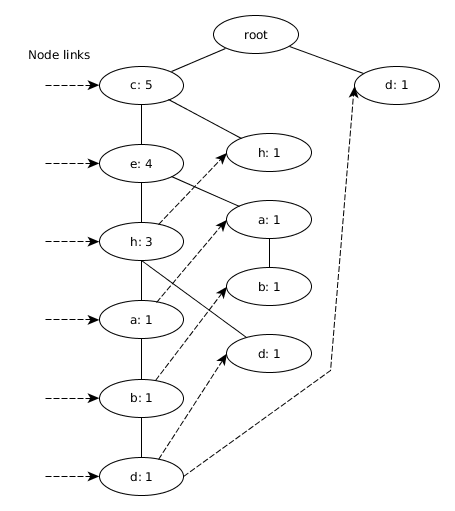
\includegraphics[scale=0.5]{fp-tree-example/fp-tree-p3.png}
	\caption{Complete FP-tree}
	\label{figure:fp-growth-example3}
\end{figure}

The dashed arrows in the FP-tree represent node links. The FP-tree maintains a table of linked lists for each distinctly named item. Whenever a node is added to the FP-tree, a pointer to that node is also added to the linked list corresponding to that nodes label. 